\chapter{Results and Discussion} \label{Results and Discussion}

The project was completed and successfully achieved it's objective of scraping and collecting the cow dung off the ground, improving collection speed and efficiency, and improved hygiene. The project achieved low collecting time that are comparable to it's expensive electrical counterparts, while having low cost of manufacturing as well as operation. The collection time improved by a huge margin as compared to conventional scraping techniques.

The most challenging part of this project after assembly was to set up the best angle of attack for the front scraper. With reference to our synthetic calculations we set it up at 45º, but in real world test it was found out the most optimised angle of attack is 60º, when the cow dung can easily drift upwards due with it's own momentum. 

The collection mechanism chain had a significant slack, this was addressed by implementing an adjustment mechanism using telescopic tubular arrangement. This allowed for easy adjustability of the slackness of the chain and easy removal of the auxiliary shafts for regular maintenance and repairs.

The use of Fusion360 for designing and analysis of this project proved to be very beneficial as it was possible to easily integrate our designs into the analysis workbench rapidly and accurately, which output precise results for reference.


\begin{figure}[H]
    \centering
    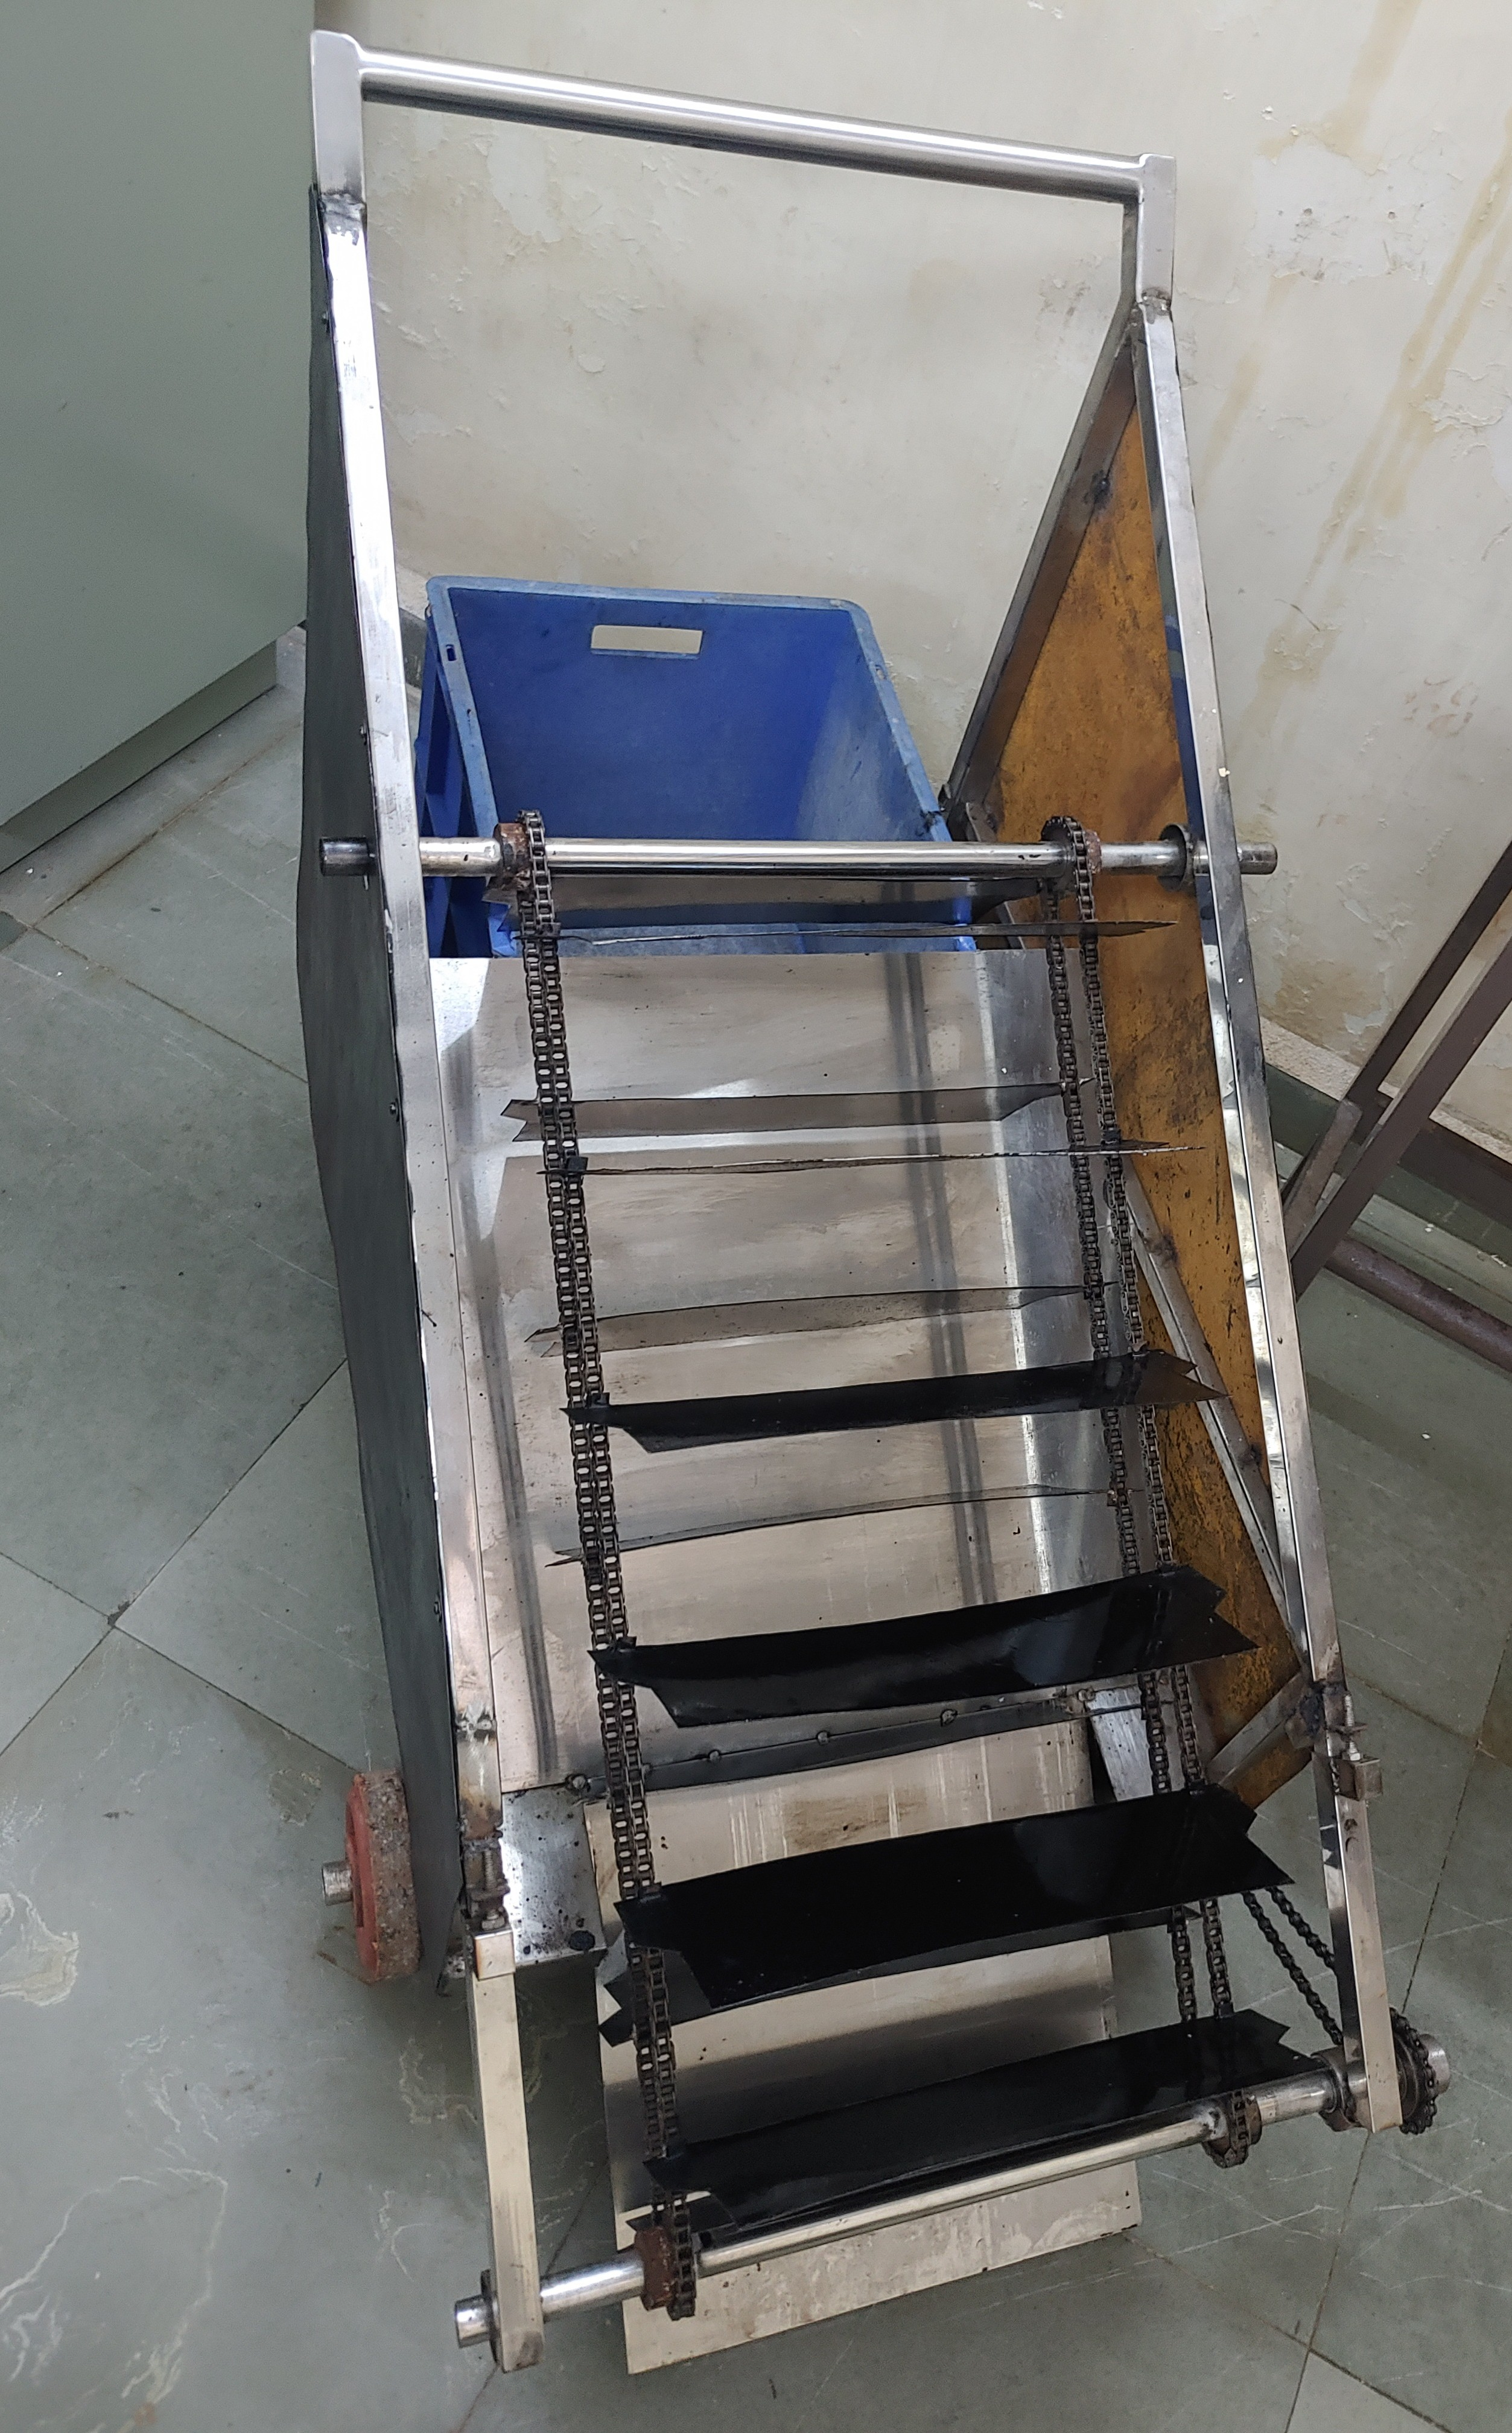
\includegraphics[scale=0.1]{with bucket 1.jpg}
    \caption{Final Prototype}
    \label{fig:final prototype 0}
\end{figure}


\pagebreak

\begin{figure}[H]
  \centering
    \begin{minipage}{0.9\textwidth}
    \centering
      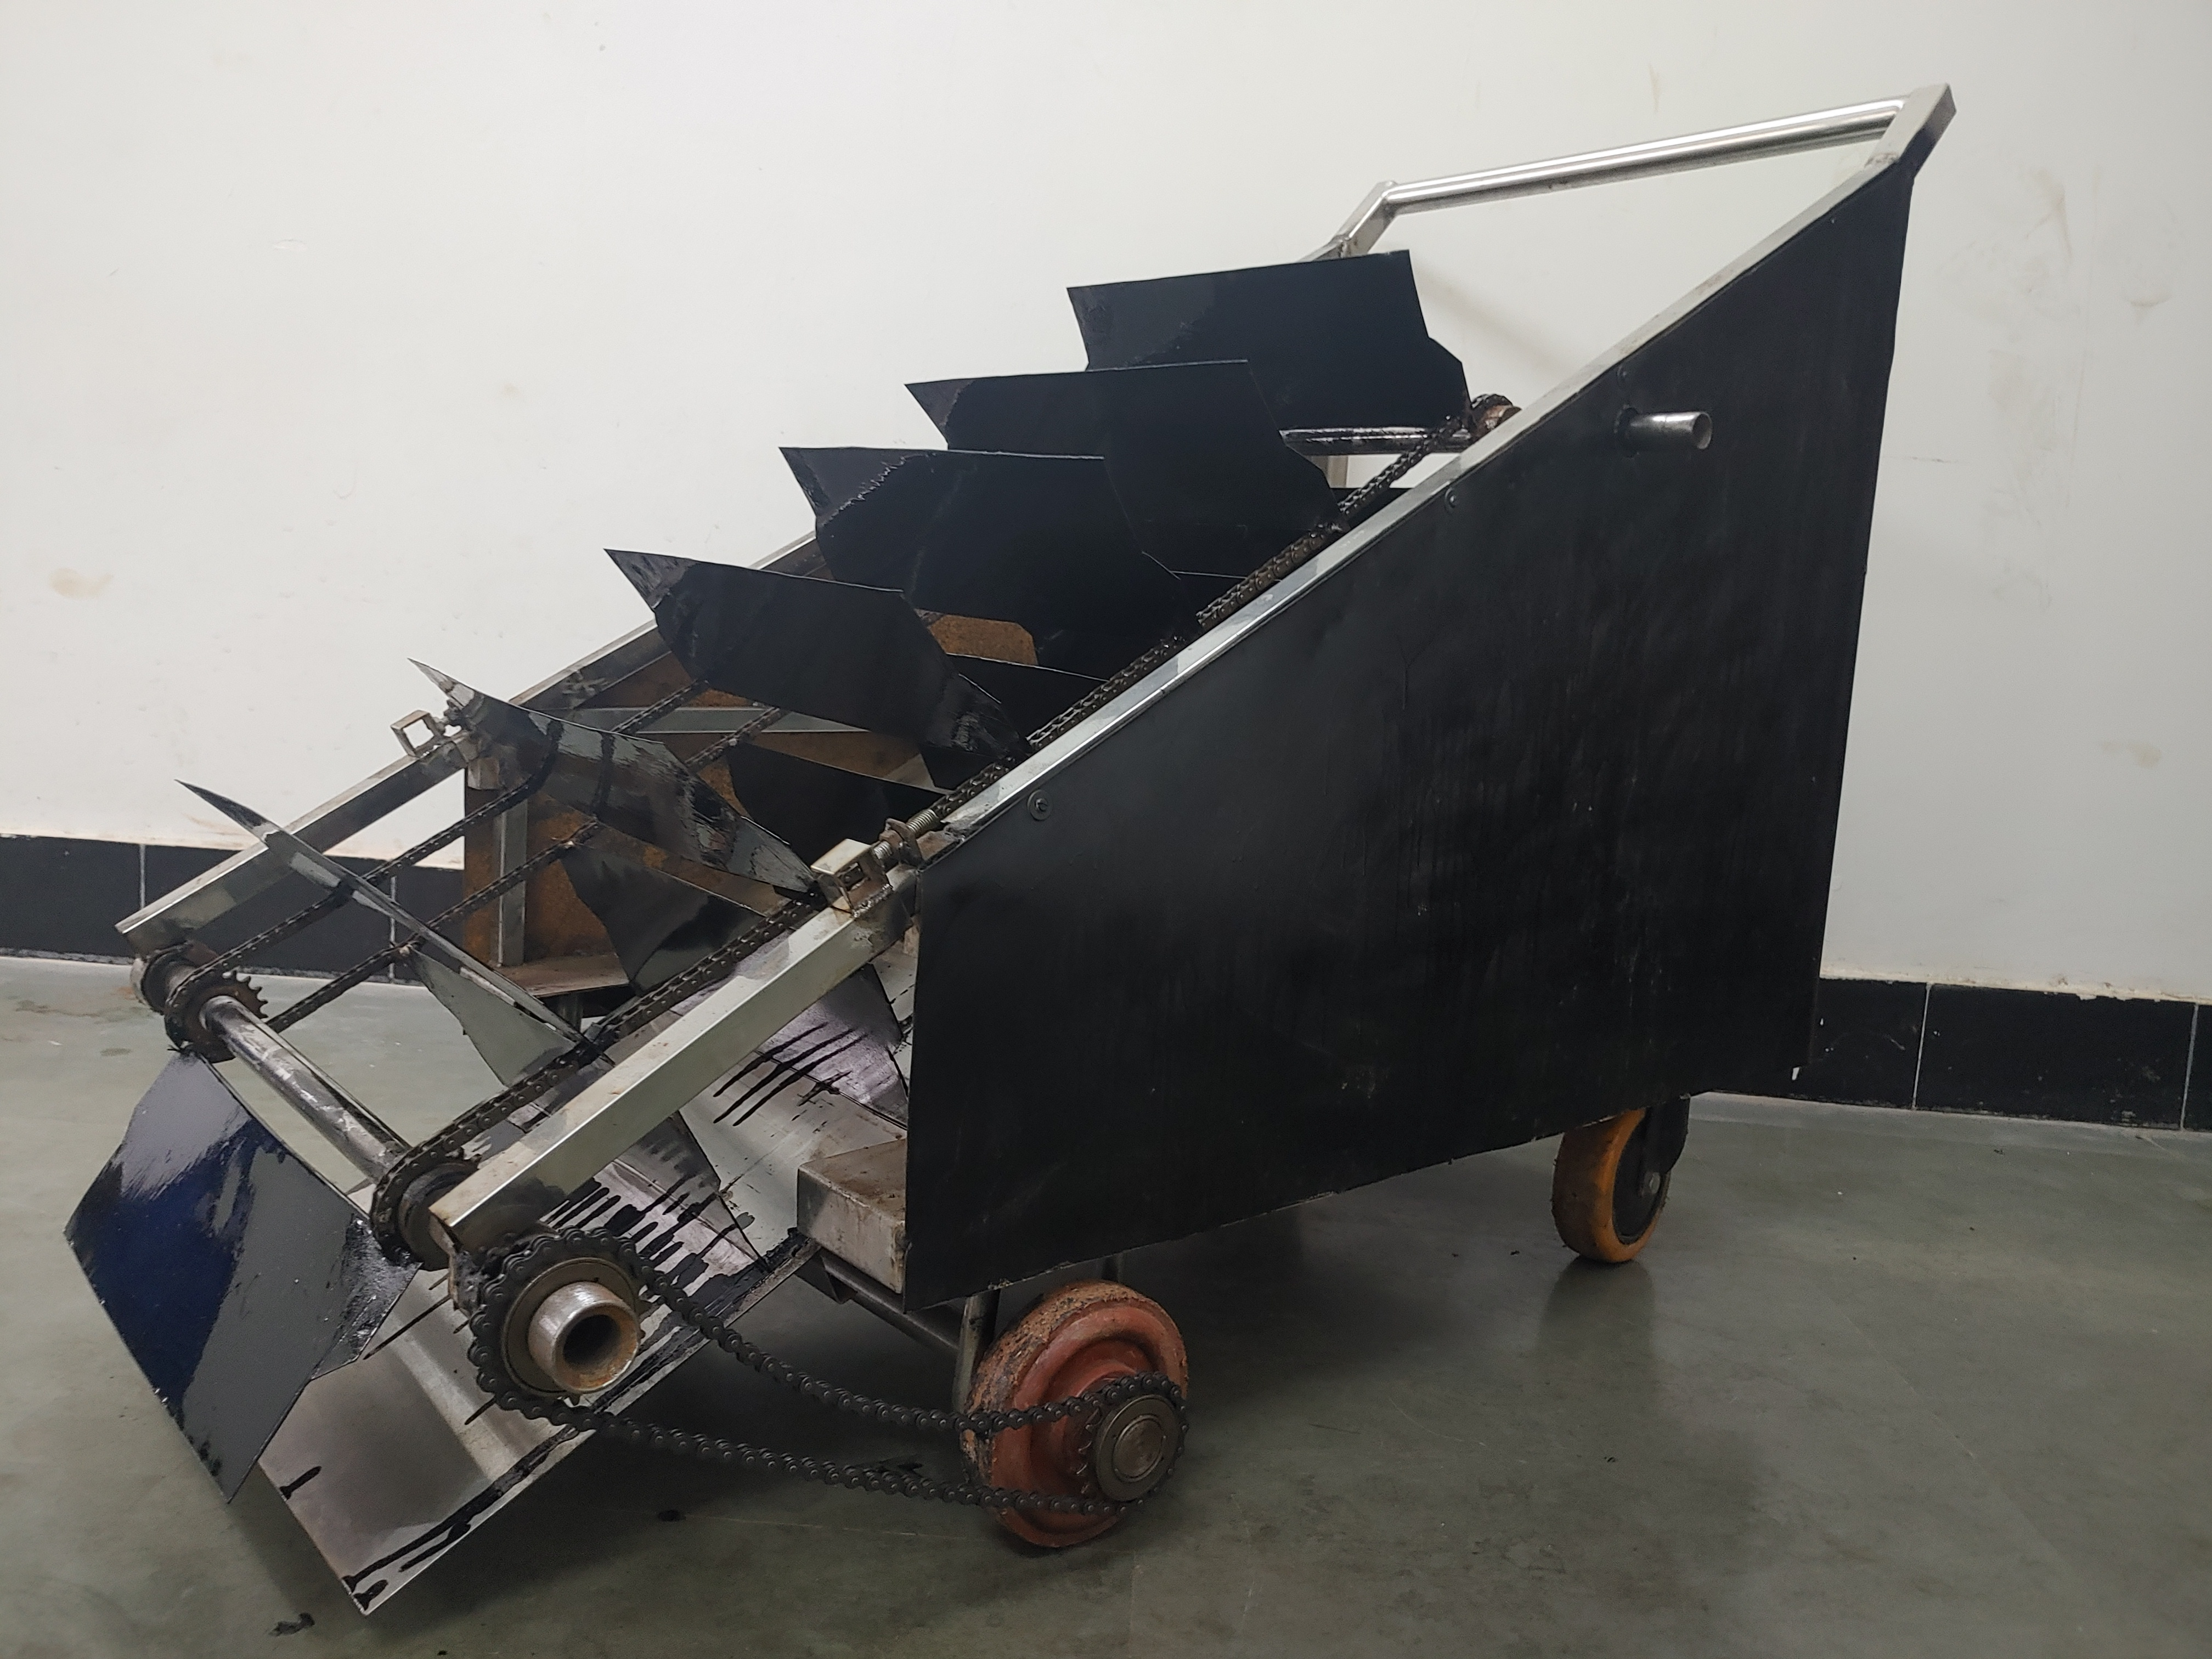
\includegraphics[width=1\textwidth]{Final Prototype.jpg}
    \end{minipage}
\hfill
    \begin{minipage}{0.9\textwidth}
    \centering
      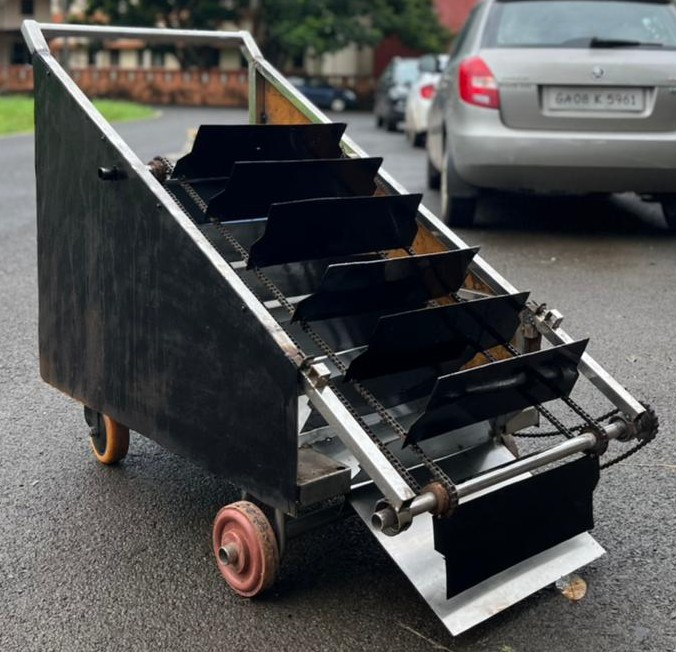
\includegraphics[width=1\textwidth]{prototype 2.jpg}
    \end{minipage}
    
    \caption{Final Prototype}
    \label{fig:Final Prototype}
\end{figure}


\pagebreak

\begin{figure}[H]
    \centering
    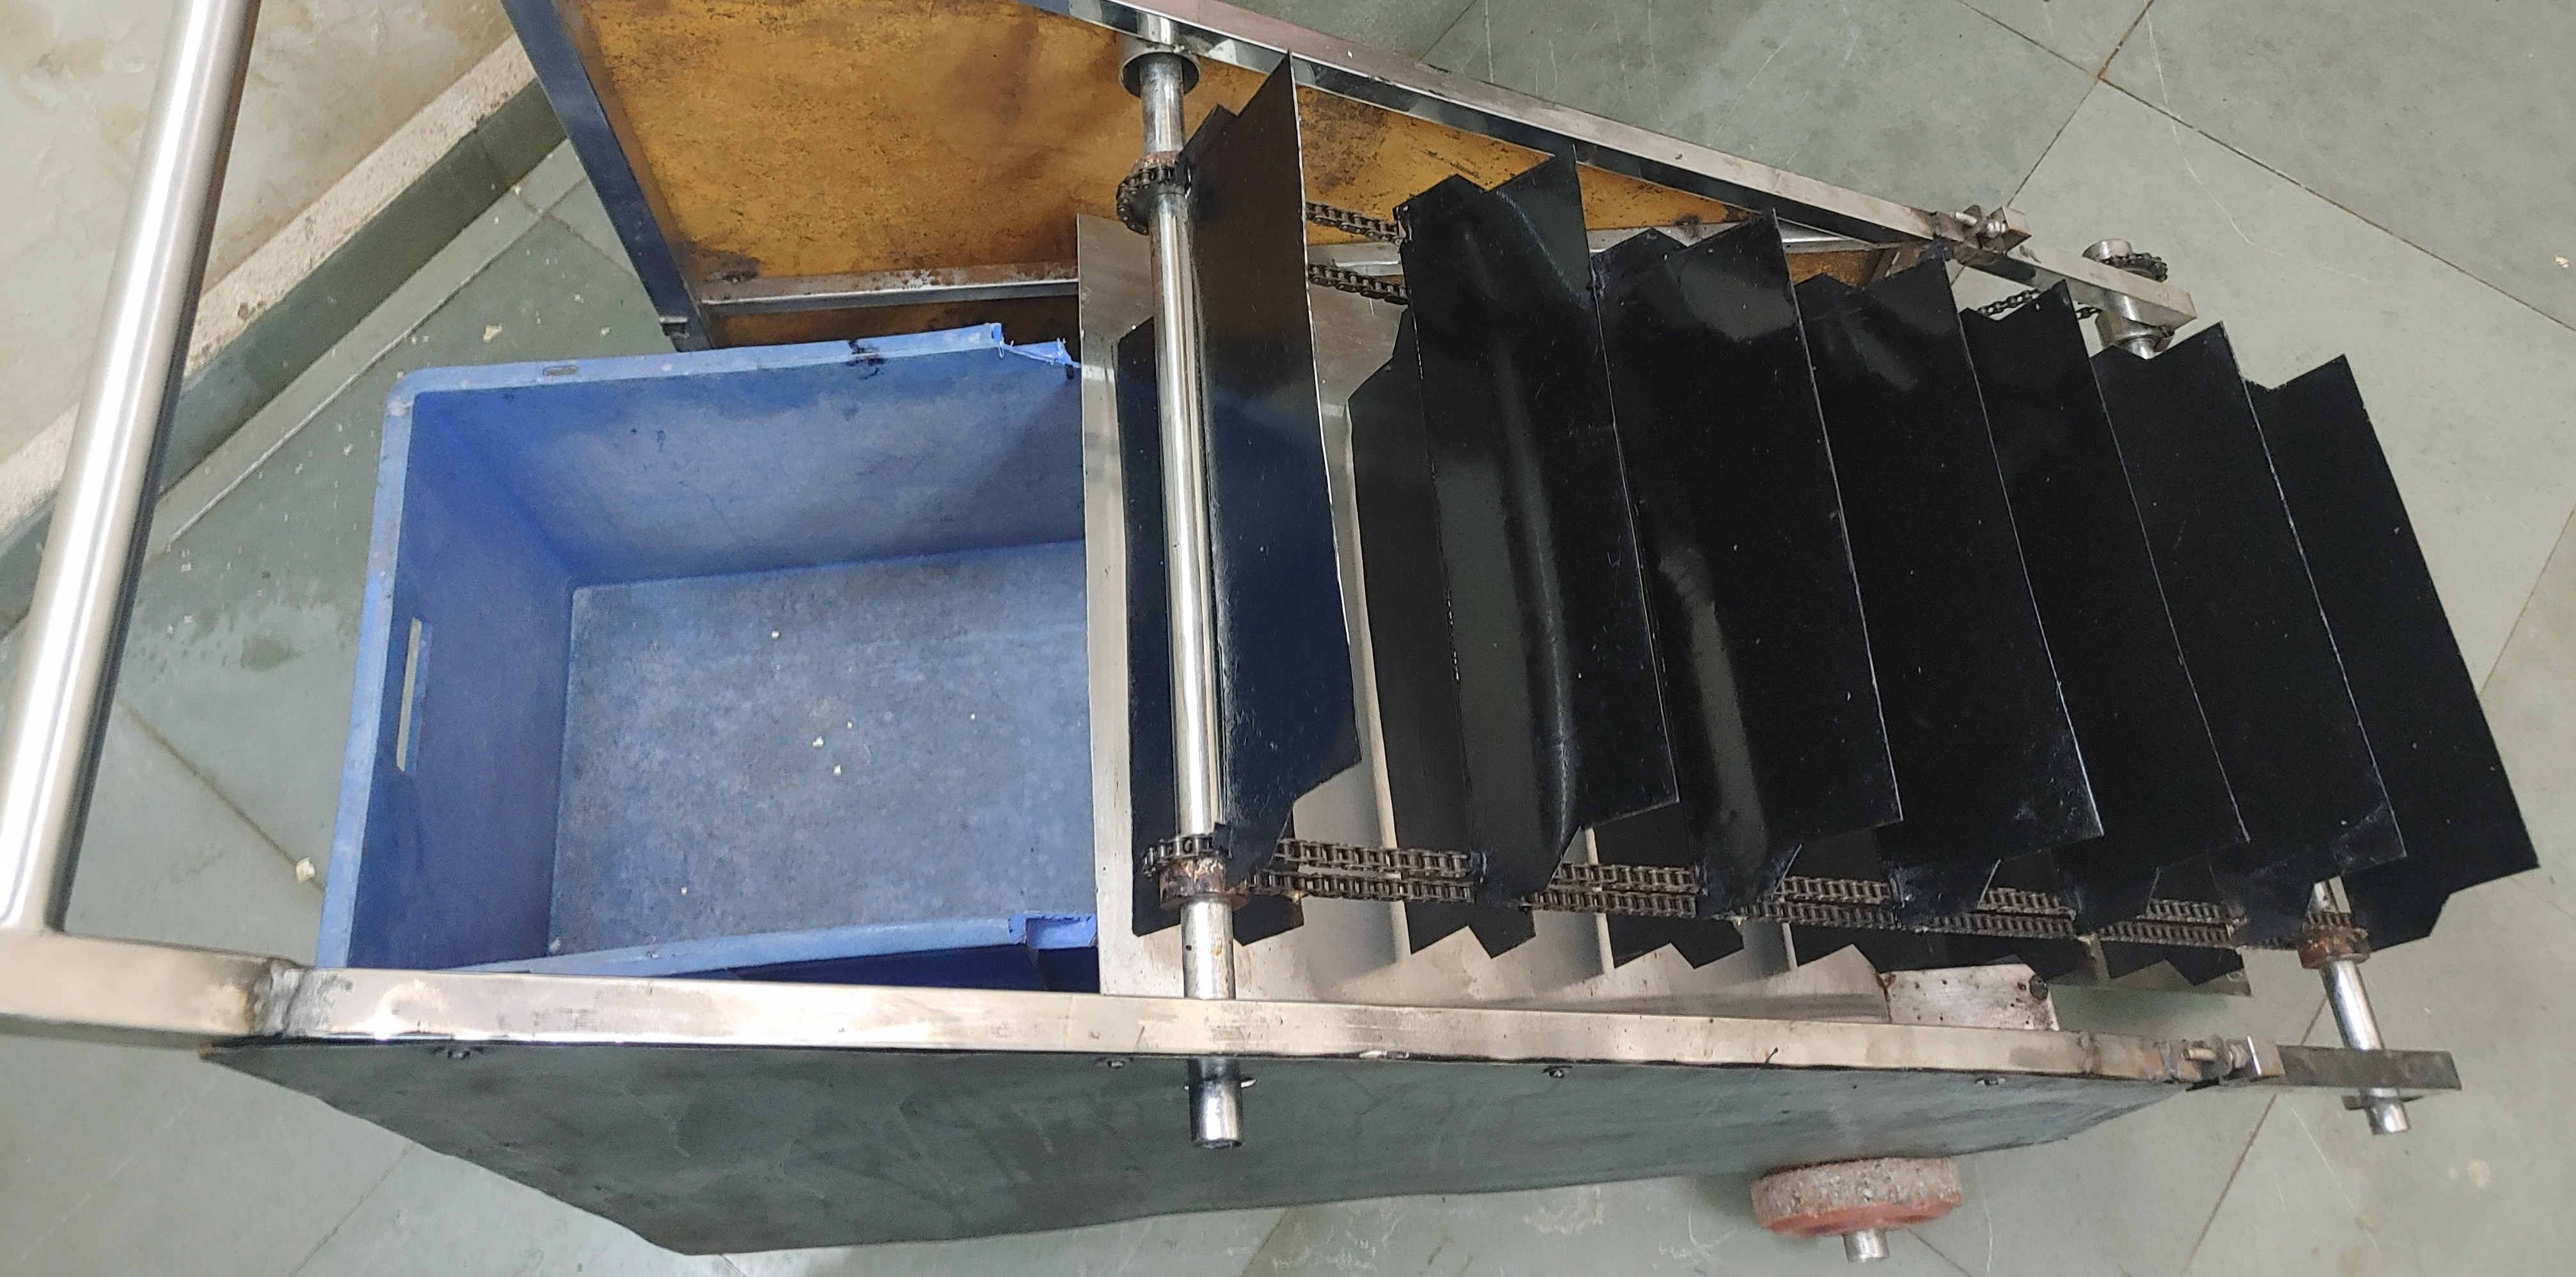
\includegraphics[scale=0.1]{with bucket 2.jpg}
    \caption{Final Prototype}
    \label{fig:prototype}
\end{figure}